\documentclass{rapportECL}

\usepackage{amsmath} 
\usepackage{amssymb} 
\usepackage{dirtree}
\usepackage{float}
\usepackage{hyperref}
\usepackage{datetime2}
\usepackage{listings}

\newcommand{\rootDirectory}{models\_creator}

\lstdefinelanguage{json}{
  basicstyle=\small\ttfamily,
  numbers=left,
  numberstyle=\tiny,
  stepnumber=1,
  numbersep=8pt,
  showstringspaces=false,
  breaklines=true,
  frame=lines,
  backgroundcolor=\color{gray!10},
  tabsize=2,
  keywordstyle=\color{blue},
  morestring=[b],
  morecomment=[l]{//},
  morecomment=[s]{/*}{*/}
}

\lstset{language=json}

\begin{document}

\reportitle{Sviluppo di una libreria Python per la creazione e gestione di sensori virtuali}


%----------- Initialisation -------------------
        
\margins 
\mytitlepage
\pagenumbering{Roman}
\toc 
\fig

\pagenumbering{arabic}


\cleardoublepage 

\chapter{Introduzione}
\label{cha:intro}

Questa libreria è stata sviluppata con l'obiettivo di agevolare il processo decisionale basato sull'analisi dei dati attraverso l'utilizzo 
di modelli di regressione lineare. Il suo scopo principale consiste nel fornire agli utenti uno strumento efficiente ed intuitivo, 
consentendo loro di generare modelli di regressione lineare tramite l'interazione con una interfaccia web dedicata. 
Gli utenti possono fornire specifici parametri di input, dai quali la libreria trae origine per la creazione dei modelli.

Questo strumento rappresenta una risorsa significativa per migliorare la capacità di prendere decisioni basate sui dati e condurre
analisi predittive accurate, contribuendo così a ottimizzare il processo decisionale in vari contesti professionali.

Questo documento è suddiviso come segue: nel capitolo~\ref{cha:import} è esposto il procedimento di importazione della libreria 
e l'installazione dei prerequisiti necessari per il corretto funzionamento della stessa. 
Nel capitolo~\ref{cha:guida}, si fornisce una guida sull'uso della libreria, includendo una breve descrizione di ogni campo di input visualizzato 
nella pagina di interazione con l'utente. Nel capitolo~\ref{cha:struttura}, viene esaminata l'organizzazione strutturale della libreria, 
con una breve illustrazione del loro contenuto di ogni file. Nel capitolo~\ref{cha:scelte}, vengono esplicate le scelte progettuali effettuate 
e il significato dei parametri utilizzati. Infine, nel capitolo~\ref{cha:funzionamento}, si offre un'analisi approfondita delle interazioni tra 
le diverse componenti del codice.

\chapter{Installazione ed esecuzione}
\label{cha:import}

Per installare la libreria, è necessario seguire attentamente i passaggi riportati di seguito:

\section*{Installazione}
\begin{enumerate}
  \item Scaricare l'intera repository dal repository GitHub ufficiale della libreria. 
  È possibile farlo tramite il comando \texttt{git clone} oppure scaricando l'archivio ZIP direttamente dal sito.
  \item Spostarsi da terminale all'interno della directory scaricata. Su Linux è possibile farlo col comando \texttt{cd \rootDirectory}
  \item Prima di procedere con l'installazione, è fondamentale verificare di avere \texttt{pip} installato nel sistema. 
  \texttt{pip} è il gestore dei pacchetti di Python e viene utilizzato per installare le dipendenze della libreria.
  \item Nel caso in cui si stia utilizzando un sistema operativo Linux, è necessario rendere il file \texttt{install.sh} eseguibile. 
  Questo può essere fatto tramite il seguente comando da terminale: \texttt{chmod +x install.sh}
  \item Eseguire il seguente comando da terminale: \texttt{./install.sh}. L'uso di questo script semplifica il processo di installazione, 
  in quanto gestirà automaticamente l'installazione di tutte le dipendenze necessarie appositamnte indicate nel file \texttt{requirements.txt}
\end{enumerate}

\section*{Esecuzione}
Per eseguire il server è necessario aprire da terminale la directory della libreria ed eseguire
il seguente comando: \texttt{python3 run.py}.



\chapter{Guida all'Utilizzo}
\label{cha:guida}

\section{Creazione dei Modelli}
\begin{enumerate}
  \item \textbf{Accedi al Server:} Utilizza il tuo browser per accedere alla pagina di creazione dei modelli della libreria, 
  collegandoti utilizzando l'indirizzo IP del server.

  \item \textbf{Login:} Per poter utilizzare la libreria è necessario effetturare l'autenticazione, fornendo username e passsword. In caso non si sia già in possesso
  di un account sarà necessario crearne uno attraverso l'apposita pagina di registrazione. 

  \begin{figure}[htp]
    \begin{minipage}{0.45\textwidth}
      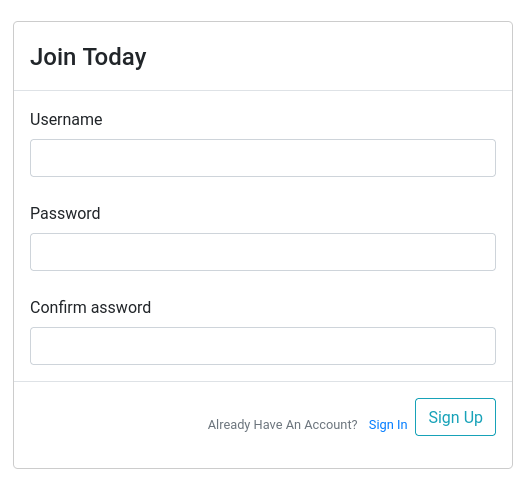
\includegraphics[width=\linewidth]{images/img2.png}
      \caption{Pagina di Registrazione}
  \end{minipage}\hfill
  \begin{minipage}{0.5\textwidth}
      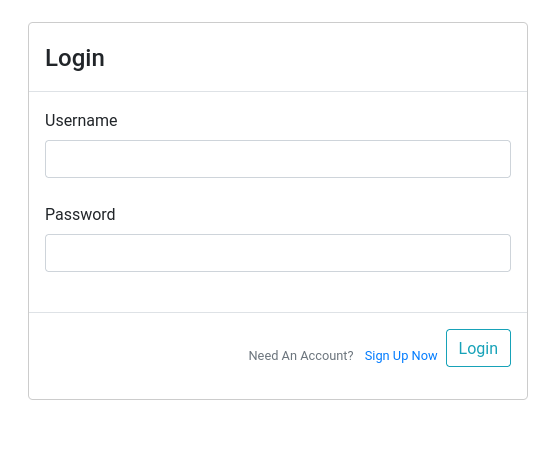
\includegraphics[width=\linewidth]{images/img3.png}
      \caption{Pagina di Login}
  \end{minipage}
  
  \end{figure}

  \item \textbf{Fornitura dei Parametri}: Per creare un modello, è necessario fornire i seguenti parametri tramite la pagina web del server:
  \begin{itemize}
    \item Scegliere tra le opzioni disponibili o introdurre un nuovo nominativo per un sensore, al quale verranno connessi i modelli oggetto della creazione imminente.
    \item Carica il file di input contenente i dati storici relativi al sensore.
    \item Carica uno o più file di output che rappresentino la variabile di risposta da prevedere.
    \item Imposta il valore  \hyperref[win]{`window'}, espresso come numero intero non negativo, che stabilirà quanti istanti temporali precedenti verranno considerati durante il processo di creazione del modello.
    \item Assegna un nome al modello. Se stai caricando più file di output, il nome verrà affiancato da un numero intero progressivo.
    \item Scegli se eseguire il test del modello. In caso affermativo, i dati verranno divisi in addestramento (80\%) e test (20\%) per la verifica della precisione.
  \end{itemize}

  \begin{figure}[htp]
    \centering
    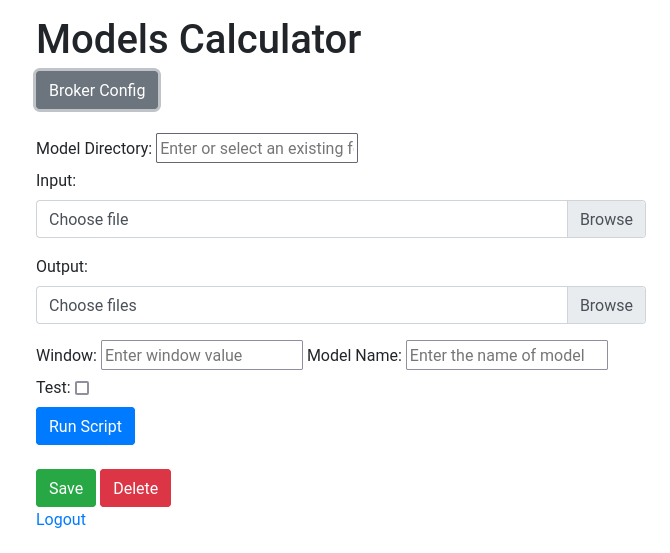
\includegraphics[width=0.75\textwidth]{images/img9.png}
    \caption{Pagina di creazione dei modelli}
  \end{figure}
  
  \item \textbf{Visualizzazione dei Risultati:} Una volta creato il modello, la libreria fornirà indicatori che valutano l'adeguatezza del modello rispetto ai dati forniti. 
  Nel caso in cui l'u tente abbia scelto di effettuare il test, verranno impiegati dei dati per valutare l'effettiva bontà delle previsioni, generando ulteriori indicatori.

  \begin{figure}[htp]
    \centering
    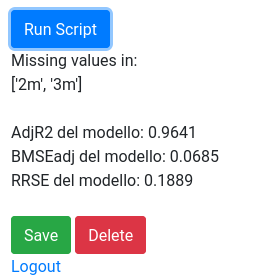
\includegraphics[width=0.25\textwidth]{images/img4.png}
    \caption{Risultati calcolo del modello}
  \end{figure}
  

  \item \textbf{Decisione di Salvare o Scartare:} A questo punto, si ha la possibilità di prendere una decisione. 
  È possibile scegliere di salvare il modello nella directory del sensore precedentemente indicata o scartarlo completamente.
  
  \item \textbf{Salvataggio con Dati Broker (opzionale):} Nel caso si decida di salvare il modello, sarà possibile creare un file di configigurazione 
  per il broker che verrà automaticamente salvato nella directory del sensore.  I parametri di configurazione del broker sono i seguenti:
  
  \begin{itemize}
    \item \texttt{Name}: Nome utente da utilizzare per connettersi al broker
    \item \texttt{Password}: Password associata al nome utente
    \item \texttt{IP del broker}: indirizzo IP che identifica il broker al quale connettersi
    \item \texttt{Topic}: Topic sul quale pubblicare le predizioni utilizzando i modelli del sensore in cui è contenuto il file di configurazione
  \end{itemize}
\end{enumerate}


\begin{figure}[htp]
  \centering
  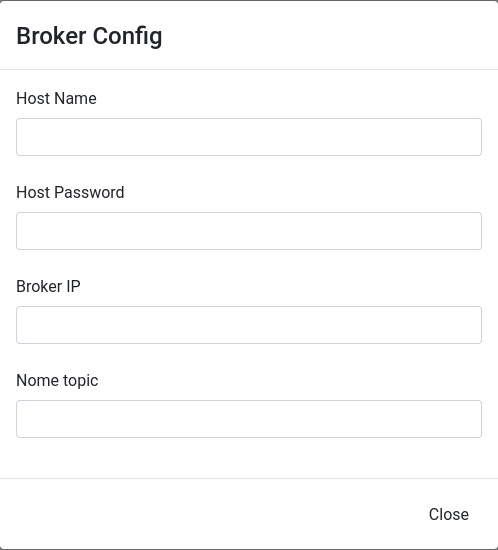
\includegraphics[width=0.5\textwidth]{images/img10.png}
  \caption{Pagina di configurazione del broker}
\end{figure}

\chapter{Struttura del codice}
\label{cha:struttura}

La struttura della repository si presenta nel seguente modo:

~\dirtree{%
.1 / (models\_creator).
.2 dir\_of\_models/.
.3 Utente/.
.4 .tmp\_models\_dir/.
.4 topic/.
.5 model.json.
.2 flaskr/.
.3 static/.
.4 main.css.
.4 index.js.
.4 models\_creator.js.
.3 templates/.
.4 index.html.
.4 login.html.
.4 register.html.
.3 \_\_init\_\_.py.
.3 views.py.
.3 login.py.
.3 models.py.
.3 uploads/.
.2 instance.
.3 site.db.
.2 ca-root-cert.crt.
.2 const.py.
.2 install.sh.
.2 models\_creator.py.
.2 reg\_class.py.
.2 reg.py.
.2 requirements.txt.
.2 run.py.
.2 subscriber.py.
.2 utils.py.
}

\section{Gestione modelli}
Il percorso di \texttt{dir\_of\_models} ospita una gerarchia di directory che riflette l'organizzazione dei modelli generati da ciascun utente. 
Ogni utente è rappresentato da una propria sottodirectory all'interno della quale si trovano i modelli da essi creati. 
È rilevabile che all'interno di queste sottodirectory utente, vi sono ulteriori suddivisioni in sottodirectory. È presente per ogni utente
una directory denominata \texttt{.tmp\_models\_dir}, la quale contiene modelli che non sono ancora stati ne salvati ne scartati, illustrando chiaramente
la loro connotazione temporanea. Per ciascun utente potrebbero esistere ulteriori sottodirectory il cui numero può variare.
Queste ulteriori directory sono finalizzate a contenere i modelli creati per ogni sensore.
Tale suddivisione consente una gestione ordinata dei vari modelli che l'utente crea nel tempo.

\section{Struttura Flask}
Flask~\cite{flask} è un framework web leggero e flessibile scritto in Python. È progettato per semplificare la creazione di applicazioni web, 
rendendo più accessibile la gestione delle richieste HTTP, delle route e delle risposte.
All'interno della directory \texttt{flaskr} troviamo l'intera struttura dell'applicazione Flask.

\begin{itemize}
  \item \textbf{static}: directory che contiene i file CSS e gli script JavaScript che vengono utilizzati per la parte front-end dell'applicazione 
  e interagiscono dinamicamente con le pagine web. Questi file sono utilizzati per personalizzare l'aspetto e il comportamento dell'app.
  \item \textbf{templates}: directory che contiene  i file HTML che vengono renderizzati sul browser dell'utente. Questi file HTML rappresentano 
  le diverse pagine web dell'applicazione e contengono il markup e i template per la visualizzazione dei dati.
  \item \textbf{uploads}: directory destinata a contenere temporaneamente i file CSV che gli utenti caricano quando eseguono il calcolo dei modelli. 
  \item \textbf{\_\_init\_\_.py}: file di inizializzazione che conferisce validità di `package' Python alla directory. 
  Inoltre, questo file incorpora il codice di configurazione, l'inizializzazione delle estensioni Flask e altre impostazioni globali dell'applicazione.
  \item \textbf{views.py}: file che definisce il comportamento dell'app in risposta alle interazioni degli utenti con la pagina web. Contiene le definizioni 
  delle route URL e delle funzioni di visualizzazione che gestiscono le richieste dell'utente e restituiscono le risposte appropriate.
  \item \textbf{login.py}: file che definisce due classi di form per l'applicazione Flask: una per la registrazione dell'utente e l'altra per l'accesso.
  \item \textbf{models.py}: file che definisce come vengono rappresentati gli utenti nel database dell'applicazione. Questo file contiene le definizioni 
  delle classi dei modelli di dati che rappresentano gli utenti e le relative informazioni nel database.
\end{itemize}

\begin{figure}[htp]
  \centering
  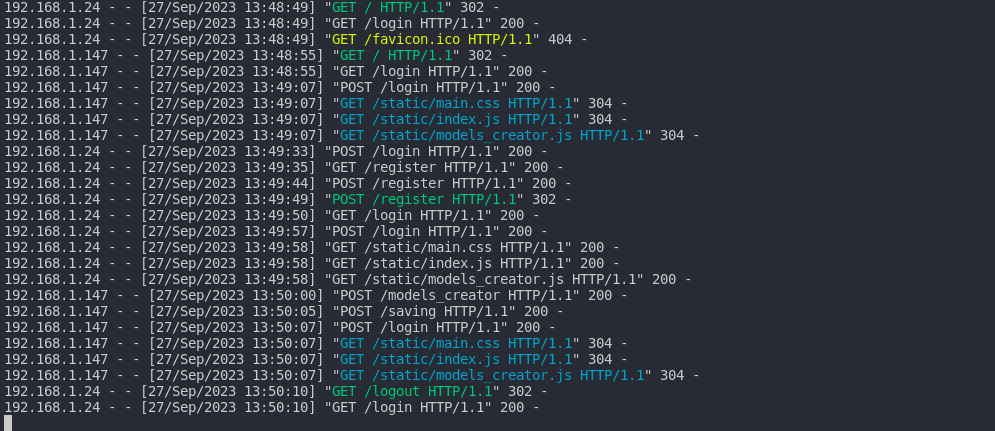
\includegraphics[width=1\textwidth]{images/img7.png}
  \caption{Gestione richieste HTTP di più utenti}
\end{figure}

\section{Gestione Utenti}
All'interno della directory \texttt{instance} troviamo il database nel quale vengono memorizzati i vari utenti. Gli utenti
sono caratterizzati dai loro nomi utente unici, dalle password per l'autenticazione e da un ID unico nel database assegnato 
automaticamente durante la fase di registrazione.


\section{Strumenti di Creazione dei Modelli}
\begin{itemize}
  \item \textbf{reg\_class.py}: definizione della classe python `RegressionModel' che funge da contenitore per tutte le
  informazioni associate ad un modello, che può essere creato o importato nell'applicazione.
  \item \textbf{reg.py}: codice che si occupa della parte di calcolo e di creazione dei modelli. Questo modulo è responsabile 
  per l'implementazione delle operazioni di creazione dei modelli basati sui dati forniti dall'utente.
  \item \textbf{utils.py}: file che contiene funzioni di utilità che aiutano a formattare i file di input in modo specifico per l'applicazione. 
  Queste funzioni sono utilizzate per elaborare e preparare i dati in modo che possano essere utilizzati nel processo di creazione del modello.
  \item \textbf{models\_creator.py}: script progettato per semplificare la creazione di più modelli di regressione mediante un'unica esecuzione. 
  Utilizza la libreria argparse~\cite{argparse} per accettare input da riga di comando.  Facilita l'automatizzazione della creazione di modelli, 
  consentendo agli utenti di ottimizzare il processo senza dover ripetere manualmente le stesse operazioni.
  \item \textbf{const.py}: file utilizzato per definire e dichiarare costanti che vengono utilizzate in diverse parti della libreria
\end{itemize}

\section{Iterazione col Broker}
Il file \texttt{subscriber.py} si occuperà di stabilire una connessione con un intermediario (broker) attraverso le credenziali specificate in 
un file posizionato all'interno di una directory dedicata al sensore dell'utente e ad un certificato    q. Dopo aver stabilito con successo questa connessione, il programma riceverà 
dati dal broker a cui è connesso. Questi dati verranno utilizzati per effettuare previsioni di valori utilizzando modelli preesistenti. 
Le previsioni risultanti saranno quindi inviate al topic specificato nel file di configurazione.
Questo codice fornisce un'applicazione basata sul protocollo MQTT~\cite{mqtt}, che utilizza la libreria Paho~\cite{paho} per connettersi 
a un broker MQTT, pubblicare messaggi e sottoscrivere argomenti per ricevere messaggi pubblicati.


\chapter{Dettagli implementativi}
\label{cha:scelte}

\section{Formato dei File CSV}

I dati in formato CSV devono essere strutturati seguendo un formato preciso e conforme. 
La prima riga dei file deve rappresentare l'intestazione, delineando i contenuti delle colonne, mentre la prima colonna è riservata ai timestamps, 
i quali devono essere accuratamente organizzati in linea con le indicazioni fornite.
\begin{enumerate} 
  \item \textbf{Formato ISO:}
  \begin{itemize}
    \item Esempio: \DTMdisplaydate{2023}{08}{10}{-1} \DTMdisplaytime{15}{30}{00}
    \item Formato: YYYY-MM-DD HH:MM:SS
  \end{itemize}
  \item \textbf{Formato europeo:}
  \begin{itemize}
    \item Esempio: 10/08/2023 15:30:00
    \item Formato: DD/MM/YYYY HH:MM:SS
  \end{itemize} 
\end{enumerate}

(Nota: è possibile tralasciare i secondi, se necessario)

\section{Matrice MxDxH}

La matrice in esame è stata progettata al fine di rappresentare l'intero arco temporale annuale, compresi i mesi, i giorni e le fasce orarie, 
mediante l'utilizzo di valori discreti espressi in forma binaria. 
La struttura matriciale è costituita da un totale di 12 colonne corrispondenti ai mesi dell'anno, 31 colonne assegnate 
ai giorni rilevanti in ciascun mese e ulteriori 24 colonne riservate alle differenti fasce orarie. 
Ciascun istante temporale sarà sottoposto a un processo di trasposizione nella forma di una sequenza binaria, 
la quale troverà collocazione all'interno di una singola riga all'interno della struttura matriciale così concepita.
 
\begin{table}[h]\centering
  \begin{tabular}{|*{14}{c|}}
  
  \hline
  1m & ... & 8m & 12m & 1d & ... & 10d & ... & 31d & 00h & ... & 15h & ... & 23h\\
  \hline
  0 & 0 & 1 & 0 & 0 & 0 & 1 & 0 & 0 & 0 & 0 & 1 & 0 & 0\\
  \hline
  
  \end{tabular}
  
  \caption{MxDxH di \DTMdisplaydate{2023}{08}{10}{-1} \DTMdisplaytime{15}{30}{00}}
\end{table}

\section{Parametro window}
\label{win}

Il parametro `window', denotato da un valore intero positivo `i', assume una funzione di rilievo nell'ambito della temporizzazione dei dati, 
contribuendo a determinare l'articolazione e l'interconnessione degli istanti temporali all'interno di un contesto sequenziale.

Nel caso in cui il parametro `window' sia settato a 0, ciascun istante temporale è trattato come un'entità isolata, distinta dalle altre in termini 
di rappresentazione e di relazioni temporali. In questa prospettiva, le informazioni ad esso associate sono espresse senza coinvolgimento di 
istanti successivi o precedenti.

Contrariamente, quando il parametro `window' è definito con un valore positivo `i', esso condiziona una dinamica di aggregazione temporale. 
Ogni istante temporale, oltre a presentare i propri dati distintivi, incorpora anche i dati relativi agli `i' istanti temporali precedenti. 
Questa configurazione crea una catena sequenziale di istanti collegati, consentendo l'analisi delle tendenze temporali su un intervallo di `i' istanti. 
È da rilevare che, in situazioni in cui il numero di istanti temporali precedenti sia inferiore a `i', 
l'istante corrente potrebbe non essere incluso nell'analisi aggregata.



\begin{table}[h]
  \centering
  \begin{tabular}{|c|c|c|}

    \hline
    timestamps & Temp & Umi\\
    \hline
    2023-08-10 13:30 & 25,1 & 8\\
    \hline
    2023-08-10 15:30 & 22,1 & 12\\
    \hline
    2023-08-10 16:30 & 21,1 & 11\\
    \hline
    2023-08-10 17:30 & 20,3 & 13\\
    \hline
  
  \end{tabular}
  
  \caption{window impostato a 0}
\end{table}


\begin{table}[h]
  \centering
  \begin{tabular}{|*{5}{c|}}
  
  \hline
  timestamps & Temp & Umi & Temp-1 & Umi-1\\
  \hline
  2023-08-10 15:30 & 22,1 & 12 & 25,1 & 8\\
  \hline
  2023-08-10 16:30 & 21,1 & 11 & 22,1 & 12\\
  \hline
  2023-08-10 17:30 & 20,3 & 13 & 21,1 & 11\\
  \hline
  
  \end{tabular}
  
  \caption{window impostato ad 1}
\end{table}


\begin{table}[H]
  \centering
  \begin{tabular}{|*{7}{c|}}
  \hline
  timestamps & Temp & Umi & Temp-1 & Umi-1 & Temp-2 & Umi-2\\
  \hline
  2023-08-10 16:30 & 21,1 & 11 & 22,1 & 12 & 25,1 & 8\\
  \hline
  2023-08-10 17:30 & 20,3 & 13 & 21,1 & 11 & 22,1 & 12\\
  \hline
  
  \end{tabular}
  
  \caption{window impostato a 2}
\end{table}


\section{Manipolazione dati}
Nel processo di manipolazione di dati espressi attraverso file CSV, sarà impiegata la libreria  \texttt{pandas}~\cite{pandas}. L'operazione preliminare 
consisterà nella conversione di questi file in strutture dati di tipo DataFrame mediante l'utilizzo della funzione  \texttt{csv\_read}. 
Tuttavia, è di fondamentale importanza porre attenzione a un insieme di strategie utili atte a garantire la qualità e l'integrità dei dati, 
nonché a fornire una base solida per le analisi successive.

Tra queste strategie figura l'adozione di accorgimenti che mirano a eliminare le colonne prive di attributi numerici o, potenzialmente, 
prive di definizione, con l'obiettivo di assicurare che solo le informazioni rilevanti siano conservate all'interno dei DataFrame. 
Parallelamente, si compirà l'azione di rimozione delle righe duplicate, allo scopo di evitare duplicazioni superflue e garantire la coerenza dei dati. 
Un ulteriore passo sarà rappresentato dall'eliminazione delle righe contenenti valori non definiti, in modo da garantire l'integrità e la completezza 
dei dati destinati all'analisi.

Risulta, inoltre, essenziale considerare che l'analisi richiede l'utilizzo di due DataFrame distinti per il calcolo del modello finale. 
Al fine di garantire la congruità tra questi due elementi, sarà impiegata la funzione \texttt{alligned}. Questa misura mira a sincronizzare 
gli istanti temporali all'interno dei due DataFrame, assicurando che solo istanti comuni siano inclusi nei dati sottoposti all'analisi. 
Ciò contribuirà a evitare conflitti temporali e a ottimizzare l'omogeneità nell'analisi stessa.

\begin{table}[htp]
  \begin{minipage}{0.45\textwidth} % Prima tabella a sinistra
    \centering
    \begin{tabular}{|c|c|c|}

      \hline
      timestamps & Temp & Umi\\
      \hline
      2023-08-10 13:30 & 25,1 & 8\\
      \hline
      2023-08-10 15:30 & 22,1 & 12\\
      \hline
      2023-08-10 16:30 & 21,1 & 11\\
      \hline
      2023-08-10 17:30 & 20,3 & 13\\
      \hline
    
    \end{tabular}
    
    \caption{File csv di input}
  \end{minipage}
  \hfill % Spazio tra le due tabelle
  \begin{minipage}{0.45\textwidth} % Seconda tabella a destra
    \centering
    \begin{tabular}{|c|c|}

      \hline
      timestamps & Var\\
      \hline
      2023-08-10 12:30 & 25,3\\
      \hline
      2023-08-10 13:30 & 25,1\\
      \hline
      2023-08-10 15:30 & 22,1\\
      \hline
      2023-08-10 16:30 & 21,1\\
      \hline
      
    
    \end{tabular}
    
    \caption{File csv di output}
  \end{minipage}
\end{table}

\begin{table}[htp]
  \begin{minipage}{0.45\textwidth} % Prima tabella a sinistra
    \centering
    \begin{tabular}{|c|c|c|}

      \hline
    timestamps & Temp & Umi\\
    \hline
    2023-08-10 13:30 & 25,1 & 8\\
    \hline
    2023-08-10 15:30 & 22,1 & 12\\
    \hline
    2023-08-10 16:30 & 21,1 & 11\\
    \hline
    
  
  \end{tabular}
  
  \caption{File di input dopo la funzione alligned}
  \end{minipage}
  \hfill % Spazio tra le due tabelle
  \begin{minipage}{0.45\textwidth} % Seconda tabella a destra
    \centering
    \begin{tabular}{|c|c|}

      \hline
    timestamps & Var\\
    \hline
    2023-08-10 13:30 & 25,1\\
    \hline
    2023-08-10 15:30 & 22,1\\
    \hline
    2023-08-10 16:30 & 21,1\\
    \hline
    
  
  \end{tabular}
  
  \caption{File csv di output dopo la funzione alligned}
  \end{minipage}
\end{table}


\section{Missing values}

Considerando che la matrice MxDxH è statica, è possibile che l'utente non fornisca dati sufficienti per garantire che ogni colonna di 
questa matrice sia diversa da zero. Questa situazione potrebbe generare problematiche durante il processo di elaborazione. 
Per prevenire tali problematiche, è stata adottata una strategia di default: ogni colonna della matrice priva di informazioni viene rilevata e segnalata 
all'utente. Successivamente, questa colonna viene esclusa dai dati utilizzati nell'analisi, al fine di assicurare una corretta elaborazione dei modelli.


\section{Maschera dei valori}

Al completamento del procedimento di calcolo di un modello, è possibile che il DataFrame risultante si presenti con una dimensione inferiore rispetto
a quella originale. Questa riduzione dimensionale deriva dal fatto che durante le fasi di selezione step-forward e step-backward, alcune colonne vengono 
scelte o escluse dal modello stesso. Questa dinamica introduce la complessità di adattare i dati futuri al modello stesso.

Per affrontare questa situazione, è stata introdotta una soluzione: l'implementazione di una maschera per i coefficienti. 
Questa maschera costituirà una mappatura dei valori dei coefficienti associati a ciascuna colonna del DataFrame originale. 
Pertanto, le colonne che non risultano presenti nel DataFrame finale verranno assegnate un valore di coefficiente pari a zero. Al contrario, le colonne 
selezionate, che preservano il loro valore di coefficiente precedentemente calcolato, sono riconosciute come significative nel contesto del modello. 
Questa metodologia di mascheramento dei coefficienti si traduce in un vantaggio determinante per l'adattamento dei dati futuri al modello, 
persino in presenza di variazioni dimensionali nel DataFrame.

\section{Formato dei modelli}

I modelli di previsione sono memorizzati nel formato JSON attraverso l'utilizzo della classe definita nel file \texttt{reg\_class.py}.
Questa classe è stata appositamente progettata per raccogliere i dettagli fondamentali dei modelli di regressione lineare 
tenendo traccia dei coefficienti associati alle colonne del file di input, delle medie e delle deviazioni standard di queste colonne, 
oltre alla media e alla deviazione standard dell'unica colonna del file di output e alle colonne non selezionate durante la fase di step-foreward
e backward. Infine viene indicato il valore di winodw usato per calcolare il modello.
(Nel modello non sarà presente la colonna timestamps in quanto sostituita dalla matrice MxDxH). Alcuni coefficenti saranno impostati a 0, 
questo in quanto viene rappresentata la maschera dei valori.

\begin{lstlisting}[caption={Esempio modello json creato.},label={esempio json},language=json]
  {
    "B": {
        "const": 0.0005468847767569886,
        "1m": 2929050859.3160734,
        "2m": 0.0,
        "3m": 0.0,
        "4m": 3039033727.51237,
        "5m": 9931225092.367886,
        ...
        "12m": 4736472045.944808,
        "1d": 36154595302.28574,
        ...
        "31d": 23077162313.65703,
        "00h": 2486308315.6457458,
        ...
        "23h": 0.1997236318436963,
        "Barometer_HPa": 0.0,
        "Temp__C": 0.0,
        "HighTemp__C": 0.0,
        "HeatingDegreeDays": -0.11052685874796615,
        "Barometer_HPa-1": 0.0,
        "Temp__C-1": 0.43701578124138385,
        "HighTemp__C-1": 0.0,
        "HeatingDegreeDays-1": 0.0
    },
    "calib_input_media": {
        "1m": 0.014922898358481181,
        "2m": 0.0,
        "3m": 0.0,
        "4m": 0.016083568230807494,
        "5m": 0.2153871663074117,
        ...
        "12m": 0.040043110595257836,
        "1d": 0.047587464765378874,
        ...
        "31d": 0.01881943292986238,
        "00h": 0.04211573536726911,
        ...
        "23h": 0.041618305421986405,
        "Barometer_HPa": 1014.2843143757254,
        "Temp__C": 19.519134471895207,
        "HighTemp__C": 19.706682142264963,
        "HeatingDegreeDays": 0.025987730061349697,
        "Barometer_HPa-1": 1014.2878046758415,
        "Temp__C-1": 19.519142762394296,
        "HighTemp__C-1": 19.70644171779141,
        "HeatingDegreeDays-1": 0.025995937655446857
    },
    "calib_input_stdev": {
        "1m": 0.1212494300378763,
        "2m": 1.0,
        "3m": 1.0,
        "4m": 0.12580222229621932,
        "5m": 0.4111077068511333,
        ...
        "12m": 0.19606847526564067,
        "1d": 0.21290057719171604,
        ...
        "31d": 0.13589257839688937,
        "00h": 0.2008615070943291,
        ...
        "23h": 0.1997236318436963,
        "Barometer_HPa": 5.316383422851651,
        "Temp__C": 7.47267783333523,
        "HighTemp__C": 7.514185801621021,
        "HeatingDegreeDays": 0.04416205072783581,
        "Barometer_HPa-1": 5.314296827667562,
        "Temp__C-1": 7.474440375604089,
        "HighTemp__C-1": 7.5157614528587775,
        "HeatingDegreeDays-1": 0.04417438440474232
    },
    "calib_output_media": 21.24883128834356,
    "calib_output_stdev": 8.274022377012576,
    "unselected_columns": [
        "2m",
        "3m",
        "Barometer_HPa",
        "Temp__C",
        "HighTemp__C",
        "Barometer_HPa-1",
        "HighTemp__C-1": 0.0,
        "HeatingDegreeDays-1": 0.0
    ],
    "window": 1
  }
        
  \end{lstlisting}
  

\chapter{Funzionamento}
\label{cha:funzionamento}

\section{Registrazione ed autenticazione}
Per poter interagire con la libreria, è necessario essere in possesso di un account. Qualora l'utente non disponga di un account, 
sarà possibile procedere con la registrazione, la quale richiederà un `username' e una `password' (con la necessità di confermare quest'ultima). 
Una volta inseriti l'username e la password, il sistema eseguirà una ricerca all'interno del database per verificare la corrispondenza delle credenziali.
Se le credenziali fornite risultano essere corrette, sarà possibile instaurare interazioni con la libreria. 
Tuttavia, nel caso in cui non emerga alcuna corrispondenza nel database in relazione alle informazioni fornite, 
l'utente verrà invitato a reinserire le proprie credenziali. 

\section{Iterazione Server e Creazione dei modelli}

Il server Flask implementa il processo di creazione dei modelli di regressione lineare mediante l'utilizzo dello script \texttt{models\_creator.py}. 
L'interfaccia web di Flask agevola la configurazione dei parametri essenziali volti a garantire il corretto funzionamento di tale script. 
I file caricati attraverso questa interfaccia, vengono rinominati come `input.csv' e `st1\_output.csv' (il valore aumenta progressivamente in base al numero dei file di output)
e vengono temporaneamente salvati all'interno della directory \texttt{uploads}.
Lo script interagirà con questa directory, dalla quale estrarrà i file di input necessari per la creazione del modello.
Al termine dell'esecuzione, lo script salva i modelli creati nella sottodirectory dell'utente chiamata \texttt{.tmp\_models\_dir}.

\section{Calcolo del modello}
Il processo di calcolo del modello si attua mediante l'invocazione della funzione \texttt{make\_regression} contenuta nel file \texttt{reg.py}. 
Questa procedura riceve in ingresso i due DataFrame derivanti dalle fasi di trattamento dati precedentemente delineate. 
In tale funzione, è osservabile la presenza di un parametro denominato `test', che se configurato a `True', 
consente la suddivisione dei dati in un set di addestramento (train) costituente l'80\% e un set di test del 20\%.  Il calcolo dei modelli
avviene secondo un accurata scelta delle colonne seguendo i metodi della libreria stepwise-regression~\cite{stepwise-regression}. 
Successivamente reintroduciamo tutte le colonne della matrice MxDxH non selezionate dalla regressione, e creiamo il modello mediante l'utilizzo della libreria statsmodels
~\cite{statsmodels}. 
Dopo la creazione, è possibile tramite il parametro `test' verificare che le predizioni siano accettabili. In conclusione, viene restituito un oggetto RegressionModel definito 
dalla classe \texttt{RegressionModel} nel file \texttt{reg\_class.py} che rappresenterà il modello creato.

\subsection{Stepwise-regression}
L'approccio stepwise alla regressione lineare procede in due fasi principali: forward e backward. Inizialmente, inizia con un modello vuoto e 
aggiunge iterativamente le variabili predittive una alla volta, valutando l'effetto di ciascuna aggiunta sulla qualità del modello. 
Successivamente, potrebbe rimuovere variabili che non contribuiscono in modo significativo al modello.
Il processo di aggiunta e rimozione continua fino a quando il modello raggiunge un miglioramento minimo del coefficiente di determinazione.


\section{Salvataggio dei Modelli}
Al termine dell'esecuzione, verrano mostrati all'utente degli indicatori che daranno un'idea della qualità delle previsioni del modello creato.
A questo punto l'utente potra decidere se scartare o se salvare il modello. Nel primo caso verrà eliminato il modello dalla directory che lo contiene, mentre nel 
secondo caso verrà spostato nella directory del sensore precedentemente scelta.

\section{Configurazione Broker}
L'utente autenticato ha la possibilità di selezionare la directory del sensore e configurare il broker in qualsiasi momento tramite l'apposito modulo. 
Una volta premuto il pulsante `Salva', il file di configurazione viene generato automaticamente all'interno della directory del sensore. 
Se esisteva già un file di configurazione precedente, questo verrà sovrascritto con il nuovo.
\bibliographystyle{plain}
\bibliography{bibliography}

\end{document}